% This LaTeX was auto-generated from MATLAB code.
% To make changes, update the MATLAB code and export to LaTeX again.

\documentclass{article}

\usepackage[utf8]{inputenc}
\usepackage[T1]{fontenc}
\usepackage{lmodern}
\usepackage{graphicx}
\usepackage{color}
\usepackage{hyperref}
\usepackage{amsmath}
\usepackage{amsfonts}
\usepackage{epstopdf}
\usepackage[table]{xcolor}
\usepackage{matlab}

\sloppy
\epstopdfsetup{outdir=./}
\graphicspath{ {./Note_Detection_images/} }

\matlabmultipletitles

\begin{document}

\matlabtitle{Определение нот}

\begin{par}
\begin{flushleft}
Начало программы
\end{flushleft}
\end{par}

\begin{par}
\begin{flushleft}
Очистка Workspace
\end{flushleft}
\end{par}

\begin{matlabcode}
clear all
close all
\end{matlabcode}



\vspace{1em}
\begin{par}
\begin{flushleft}
Определяю таблицу частот и нот
\end{flushleft}
\end{par}

\begin{par}
\begin{flushleft}
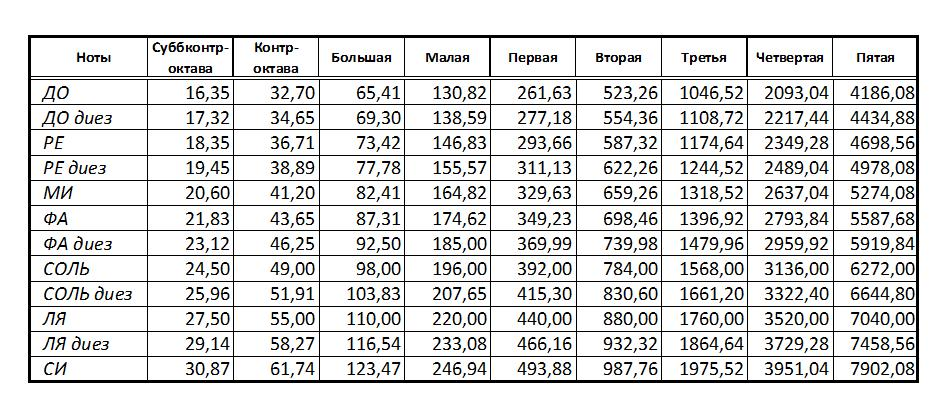
\includegraphics[width=\maxwidth{55.09282488710487em}]{image_0}
\end{flushleft}
\end{par}

\begin{matlabcode}
% Большая октава
Tab_F_1 = [65.41  69.3  73.42  77.78  82.41  87.31  92.5  98  103.83  110  116.54  123.47];

% Математически получаем частоты остальных октав
k = 2.^(0:6);
Tab_F = k' .* repmat(Tab_F_1, 7, 1);

figure (1)
plot(Tab_F)
xlabel("Octave number")
ylabel("Frequency")
title("Frequency of notes as a function of octave number")
\end{matlabcode}
\begin{center}
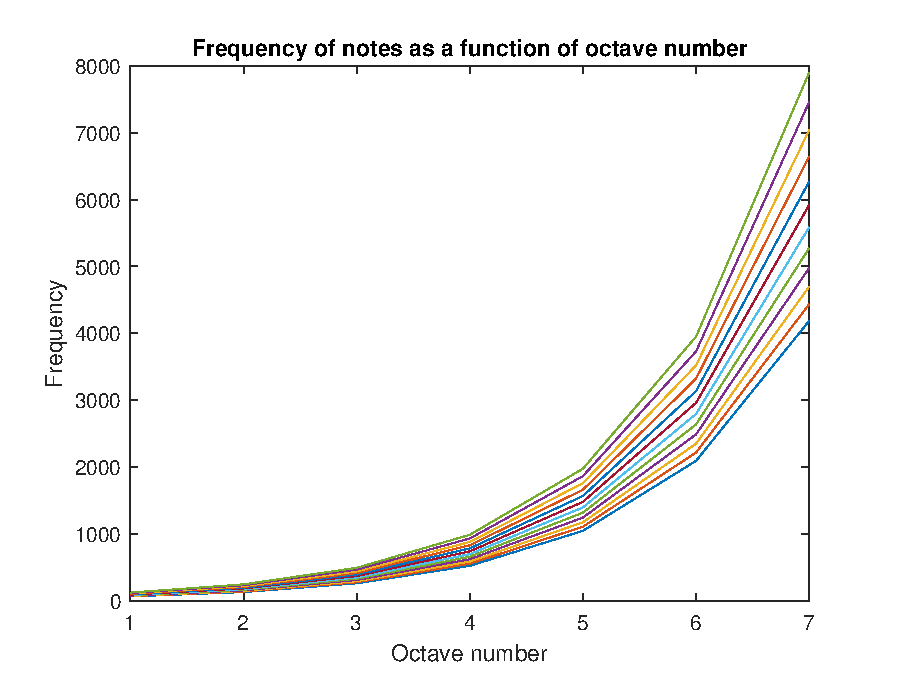
\includegraphics[width=\maxwidth{56.196688409433015em}]{figure_0.eps}
\end{center}

\begin{par}
\begin{flushleft}
Очистка от ненужного
\end{flushleft}
\end{par}

\begin{matlabcode}
clear Tab_F_1  k
\end{matlabcode}


\begin{par}
\begin{flushleft}
Определяю матрицу сумм, в которую из спектра я буду складывать составляющие по частотам каждой ноты. КАждая ячейка соответствует мощности в спектре конкретной ноты конкретной октавы.
\end{flushleft}
\end{par}

\begin{matlabcode}
M = zeros(7, 12);
\end{matlabcode}



\vspace{1em}
\begin{par}
\begin{flushleft}
Загрузка аудиофайла с 60 нотами подряд
\end{flushleft}
\end{par}

\begin{matlabcode}
path = 'D:\Desktop\Studie\Diploma\Audio data\wav\60 нот.wav';
[y, Fs] = audioread(path);

z = y(:,1);
figure (1)
spectrogram(z,6000, 2000,6000,Fs,'yaxis')
title('Sound spectrogram')
ylim([0 3])
\end{matlabcode}
\begin{center}
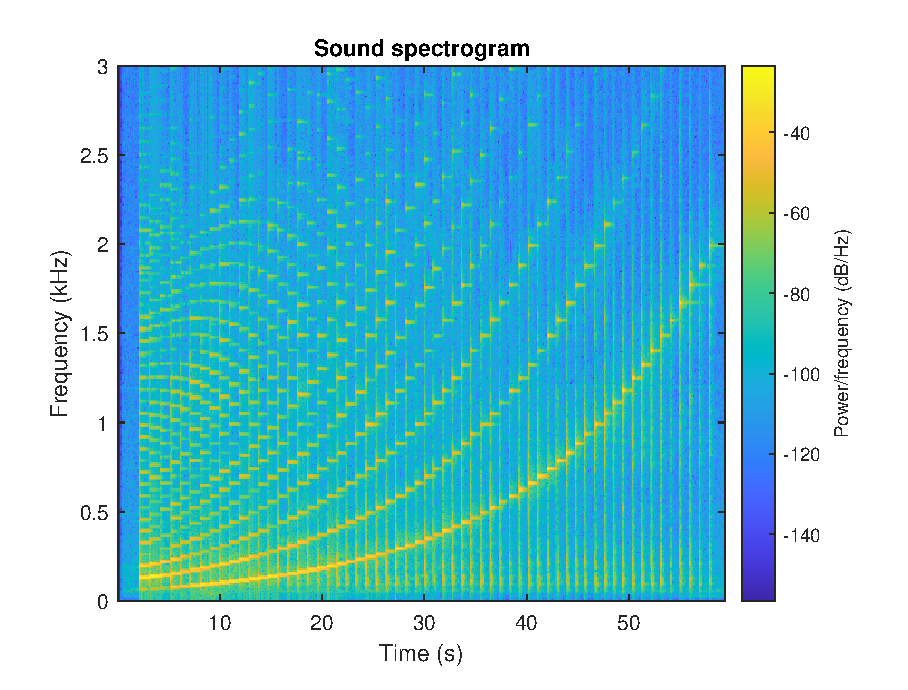
\includegraphics[width=\maxwidth{56.196688409433015em}]{figure_1.eps}
\end{center}

\begin{par}
\begin{flushleft}
Очистка от ненужного
\end{flushleft}
\end{par}

\begin{matlabcode}
clear y path
\end{matlabcode}


\begin{par}
\begin{flushleft}
Определяю максимальную пачку отчетов спектр которого я могу брать для анализа, что бы заметить самую быструю ноту.
\end{flushleft}
\end{par}

\begin{matlabcode}
bpm = 120;          % 120 таков в минуту
bps = bpm/60;       % или 2 доли в секунду
t_d = 1/bps;        % что есть 0.5сек на долю
Note_min = 1/16;    % Условно минимальная продолжительность ноты
                    % 1/16 доли

T_min = Note_min * t_d
\end{matlabcode}
\begin{matlaboutput}
T_min = 0.0313
\end{matlaboutput}
\begin{matlabcode}

Fs = 44100;         % При частоте дискретизации 44 100Гц получаем
Samples_num = T_min * Fs
\end{matlabcode}
\begin{matlaboutput}
Samples_num = 1.3781e+03
\end{matlaboutput}
\begin{matlabcode}

Samples_num = 1024  % С округлением в низ
\end{matlabcode}
\begin{matlaboutput}
Samples_num = 1024
\end{matlaboutput}
\begin{matlabcode}

df = Fs/Samples_num % В таком случае шаг частоты спектра 43Гц
\end{matlabcode}
\begin{matlaboutput}
df = 43.0664
\end{matlaboutput}

\begin{par}
\begin{flushleft}
Очистка от ненужного
\end{flushleft}
\end{par}

\begin{matlabcode}
clear bpm bps t_d Note_min T_min df
\end{matlabcode}


\begin{par}
\begin{flushleft}
Определение векторов "Vi" для извлечения амплитуд. АЛЬТЕРНАТИВА: находим массив "Indexes" индексов которые соответствуют нотам 
\end{flushleft}
\end{par}

\begin{par}
\begin{flushleft}
Для начала выделю участок сигнала и проинтерполирую его спектр
\end{flushleft}
\end{par}

\begin{matlabcode}
Fs = 44100;
i = 400;
S = z(i*Samples_num: (i+1)*Samples_num -1);

L = length(S);
df = Fs/L;

figure(1)
plot(abs(fft(S)))
xlim([0 20])
title("Спектр участка сигнала")
\end{matlabcode}
\begin{center}
\includegraphics[width=\maxwidth{56.196688409433015em}]{figure_2.eps}
\end{center}
\begin{matlabcode}

k_interp = Fs/length(S) - 1;
zeros_num = floor( k_interp*Samples_num );
Zer = zeros(zeros_num, 1);
S2 = vertcat (Zer, S);

L2 = length(S2);
df2 = Fs/L2;

figure(2)
plot(abs(fft(S2)))
xlim([0 20] * k_interp)
title("Спектр участка сигнала после интерполяции")
\end{matlabcode}
\begin{center}
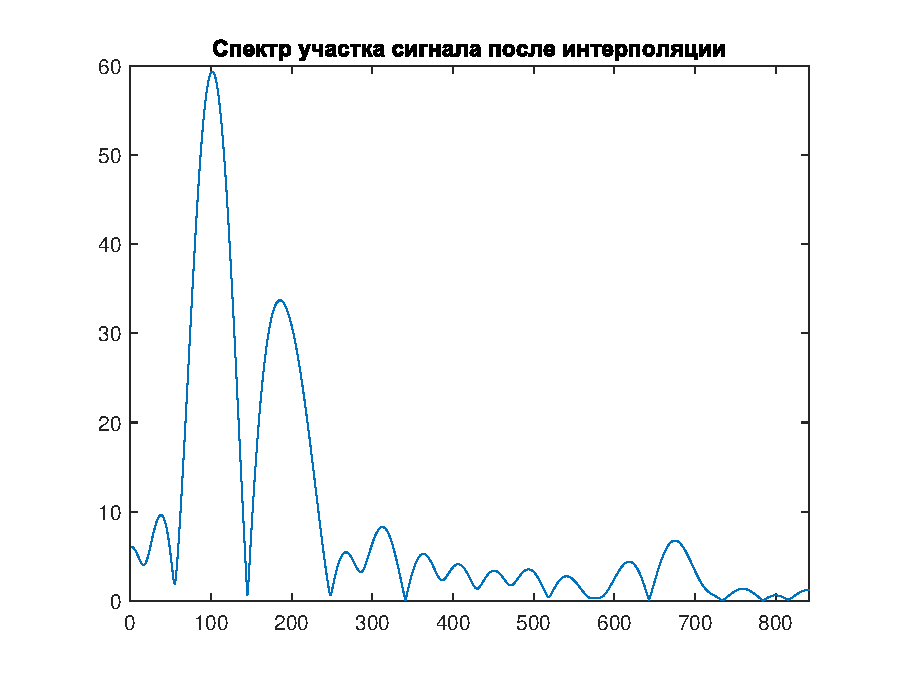
\includegraphics[width=\maxwidth{56.196688409433015em}]{figure_3.eps}
\end{center}

\begin{par}
\begin{flushleft}
Теперь, имея удобный спектр, найду индексы, которые соответствуют частотам нот
\end{flushleft}
\end{par}

\begin{par}
\begin{flushleft}
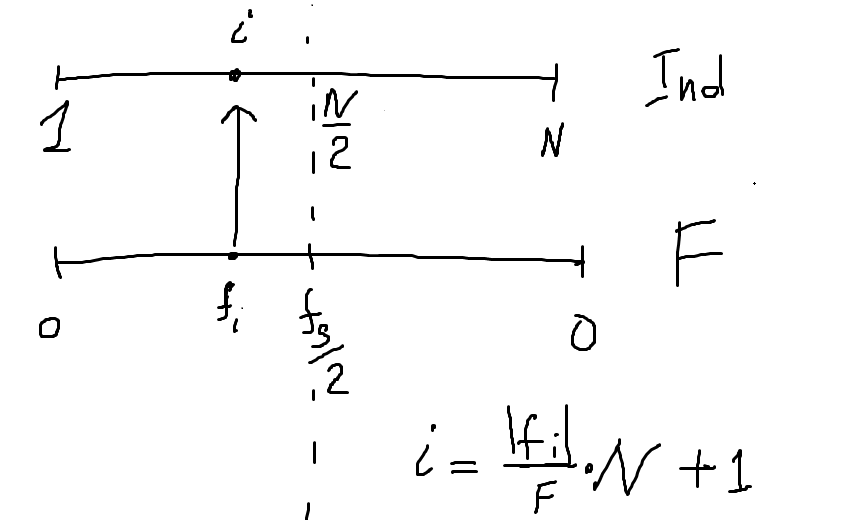
\includegraphics[width=\maxwidth{51.580531861515304em}]{image_1}
\end{flushleft}
\end{par}

\begin{matlabcode}
FlatTab_F = reshape(Tab_F.',1,[]);               % FLAT!!!
Indexes = floor(L2 * FlatTab_F / Fs + 1);


Spec = abs(fft(S2));
Spec = Spec(1:L2/2);
f = 0:df2:Fs/2-df2;


figure (3)
plot(f, Spec, FlatTab_F, Spec(Indexes), '*')
xlim([0 600])
title("Астериксами показаны амплитуды на частотах нот")
\end{matlabcode}
\begin{center}
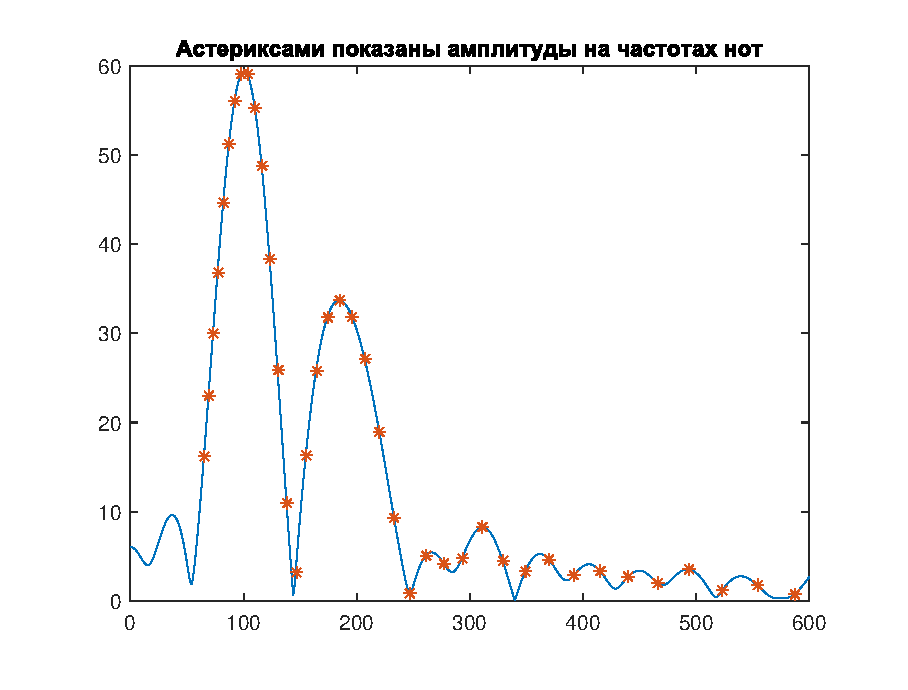
\includegraphics[width=\maxwidth{56.196688409433015em}]{figure_4.eps}
\end{center}


\begin{par}
\begin{flushleft}
Проба записи матрицы М для 1го слайса
\end{flushleft}
\end{par}

\matlabtitle{ИЗМЕНЯЙ "i" И НАБЛЮДАЙ 3Д ИЗОБРАЖЕНИЕ МАТРИЦЫ}

\begin{par}
\begin{flushleft}
i = 1...2500
\end{flushleft}
\end{par}

\begin{matlabcode}
i = 1350;
S = z(i*Samples_num: (i+1)*Samples_num - 1);

figure(1)
subplot(2,1,1)
plot(abs(fft(S)))
xlim([0 20])
title("Спектр участка сигнала")

k_interp = Fs/length(S) - 1;
zeros_num = floor( k_interp*Samples_num );
Zer = zeros(zeros_num, 1);
S2 = vertcat (Zer, S);

figure(1)
subplot(2,1,2)
plot(abs(fft(S2)))
xlim([0 20] * k_interp)
title("Спектр участка сигнала после интерполяции")
\end{matlabcode}
\begin{center}
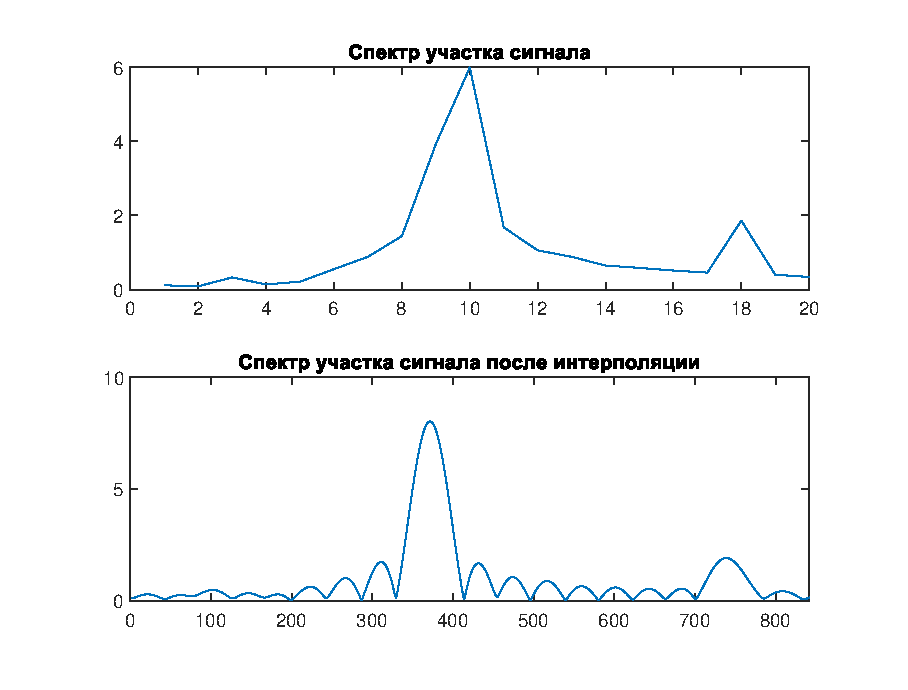
\includegraphics[width=\maxwidth{56.196688409433015em}]{figure_5.eps}
\end{center}
\begin{matlabcode}


Indexes = floor(L2 * Tab_F / Fs + 1);   % NOT FLAT!!!


Spec = abs(fft(S2));
Spec = Spec(1:L2/2);

M = Spec(Indexes);

figure(2)
mesh(M);
xlabel("Notes")
ylabel("Octaves")
title("Представление матрицы амплитуд спектра на частотах нот")
\end{matlabcode}
\begin{center}
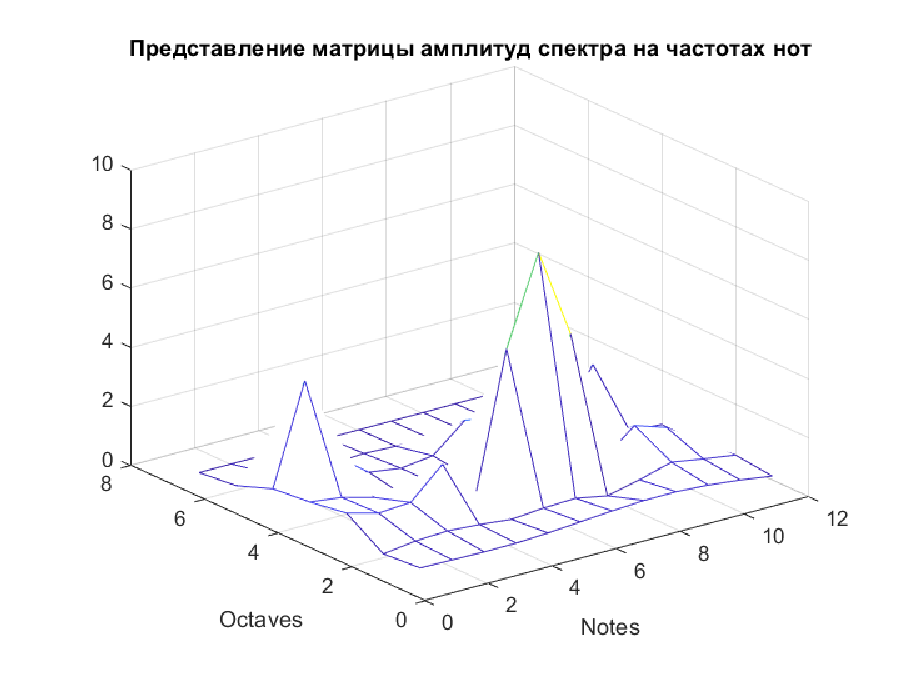
\includegraphics[width=\maxwidth{56.196688409433015em}]{figure_6.eps}
\end{center}


\begin{par}
\begin{flushleft}
Определение 1 ноты определением максимума матрицы М
\end{flushleft}
\end{par}

\begin{matlabcode}
i = 1350;
S = z(i*Samples_num: (i+1)*Samples_num - 1);

k_interp = Fs/length(S) - 1;
zeros_num = floor( k_interp*Samples_num );
Zer = zeros(zeros_num, 1);
S2 = vertcat (Zer, S);

figure(4)
plot(abs(fft(S2)))
xlim([0 20] * k_interp)
title("Спектр участка сигнала после интерполяции")
\end{matlabcode}
\begin{center}
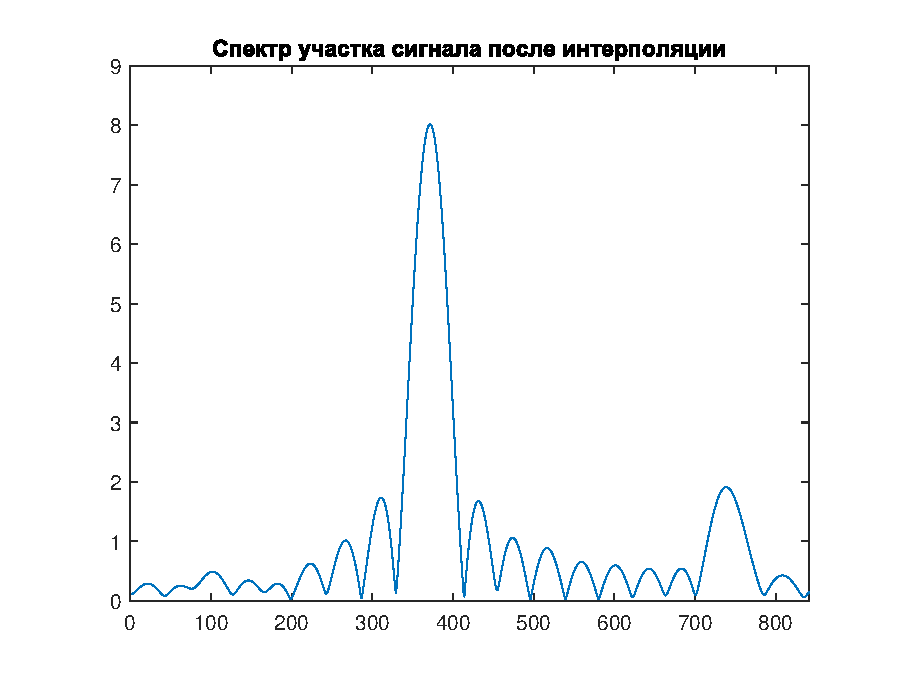
\includegraphics[width=\maxwidth{56.196688409433015em}]{figure_7.eps}
\end{center}
\begin{matlabcode}

Indexes = floor(L2 * Tab_F / Fs + 1);   % NOT FLAT!!!

Spec = abs(fft(S2));
Spec = Spec(1:L2/2);

M = Spec(Indexes);
\end{matlabcode}

\begin{par}
\begin{flushleft}
Октава и нота. ранспонировки матрицы мы идем по октавам фиксируя ноты. С транспонировкой - фиксируется октава и мы идем по нотам. 
\end{flushleft}
\end{par}

\begin{par}
\begin{flushleft}
Значит индекс = октава*12 + нота
\end{flushleft}
\end{par}

\begin{matlabcode}
[Val, Ind] = max(M',[],[1 2], 'linear')   % Нахожу индекс максимума
\end{matlabcode}
\begin{matlaboutput}
Val = 8.0162
Ind = 31
\end{matlaboutput}
\begin{matlabcode}

note_num = mod(Ind, 12)            
\end{matlabcode}
\begin{matlaboutput}
note_num = 7
\end{matlaboutput}
\begin{matlabcode}
octave_num = (Ind - note_num)/12 + 1
\end{matlabcode}
\begin{matlaboutput}
octave_num = 3
\end{matlaboutput}


\matlabheading{Определение нот композиции}

\begin{par}
\begin{flushleft}
Подготавливаем массив для нот композиции и задаем количество вырезок которые мы совершим
\end{flushleft}
\end{par}

\begin{matlabcode}
cuts = floor( length(z) / Samples_num ) - 1;    % Кол-во вірезок по времени
notes_lin = zeros(1, cuts);
\end{matlabcode}

\begin{par}
\begin{flushleft}
Заготавливаем массив нулей для интерполяции
\end{flushleft}
\end{par}

\begin{matlabcode}
k_interp = Fs/Samples_num - 1;
zeros_num = floor( k_interp*Samples_num );
Zer = zeros(zeros_num, 1);
\end{matlabcode}

\begin{par}
\begin{flushleft}
Заготавливаем массив индексов спектра для получаения амплитуд нот
\end{flushleft}
\end{par}

\begin{matlabcode}
Indexes = floor(L2 * Tab_F / Fs + 1);   % NOT FLAT!!!
\end{matlabcode}

\begin{par}
\begin{flushleft}
Находим все ноты композиции и записываем в "notes\_lin" в виде "нота*7 + октава". Такую форму дает линейная индексация от встроенной функции max.
\end{flushleft}
\end{par}

\begin{matlabcode}
for i = 1:cuts
    
    n1 = i*Samples_num;         % Задаю пределы для вырезания участка сигнала
    n2 = (i+1)*Samples_num - 1;
    
    S = z(n1: n2);              % Берем участок сигнала
    S2 = vertcat (Zer, S);      % Интерполируем спектр
    Spec = abs(fft(S2));        % Находим спектр сигнала
    M = Spec(Indexes);          % Заполняем матрицу нот
    
    [Val, Ind] = max(M',[],[1 2], 'linear');   % Нахожу индекс максимума
    
    notes_lin(i) = Ind;         % Сохраняю текущую ноту
    
    if mod(i,200) == 0
        figure(i)
        mesh(M);
        xlabel("Notes")
        ylabel("Octaves")
        title("Matrix number #" + string(i) + ". LinIndex = " + string(Ind))
    end
    
end
\end{matlabcode}
\begin{center}
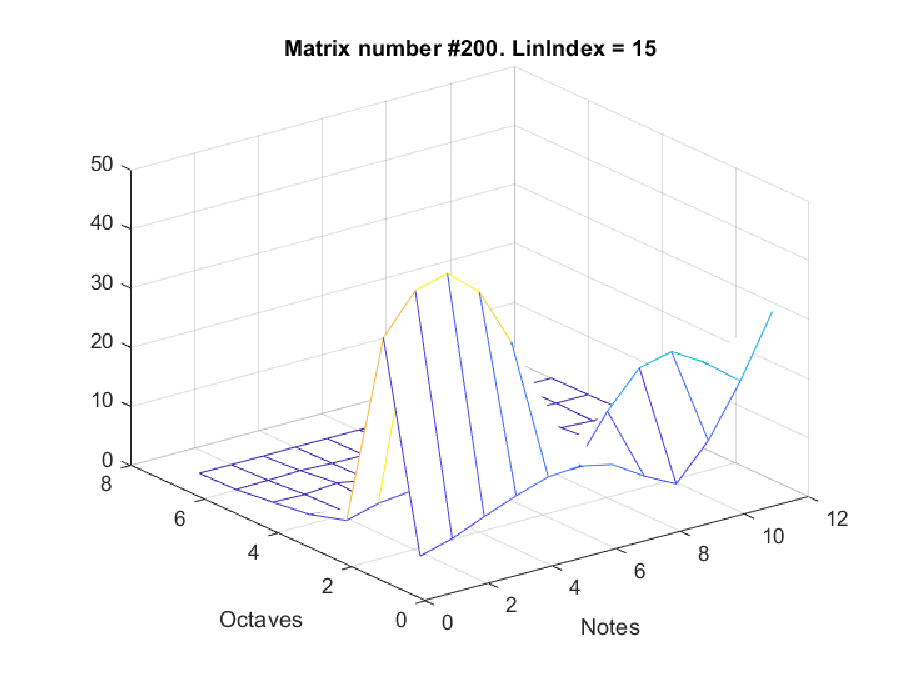
\includegraphics[width=\maxwidth{56.196688409433015em}]{figure_8.eps}
\end{center}
\begin{center}
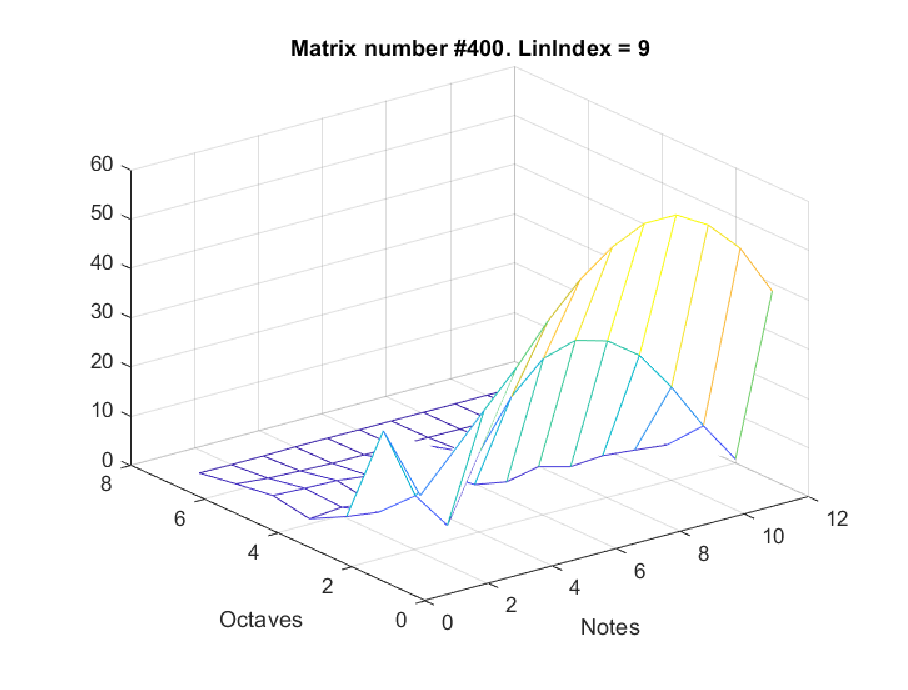
\includegraphics[width=\maxwidth{56.196688409433015em}]{figure_9.eps}
\end{center}
\begin{center}
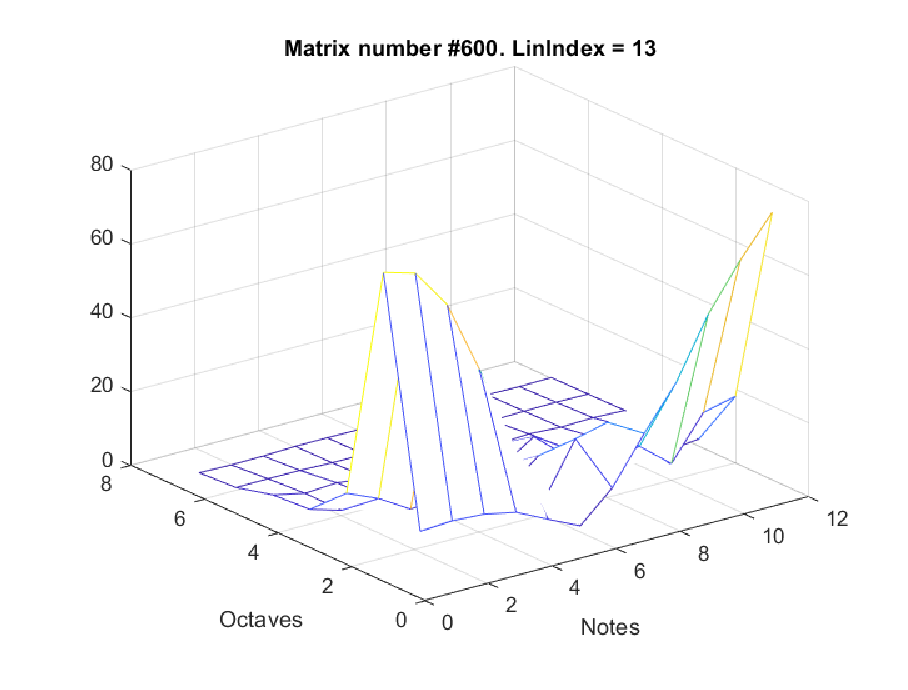
\includegraphics[width=\maxwidth{56.196688409433015em}]{figure_10.eps}
\end{center}
\begin{center}
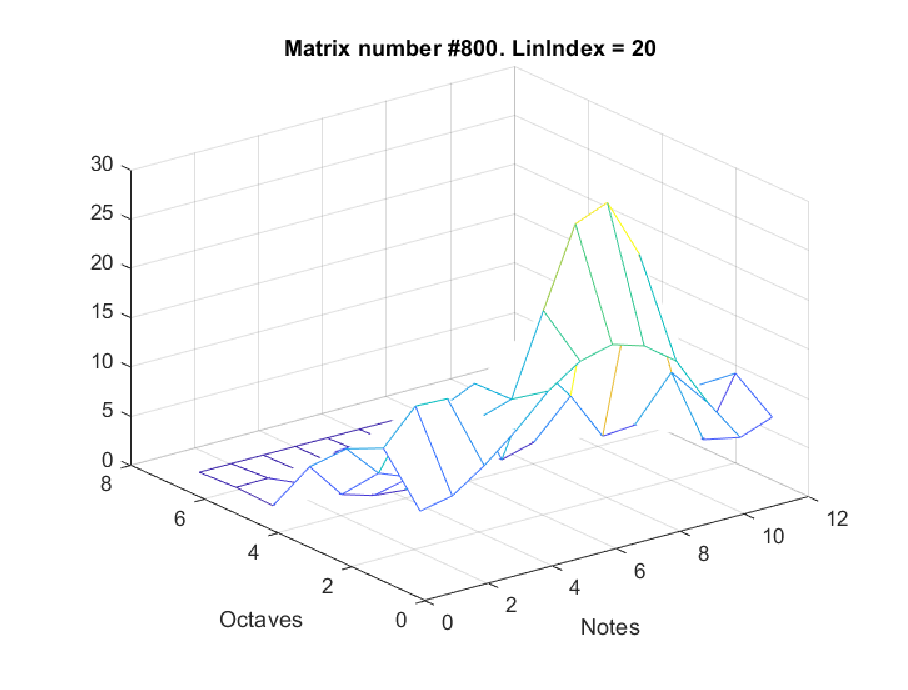
\includegraphics[width=\maxwidth{56.196688409433015em}]{figure_11.eps}
\end{center}
\begin{center}
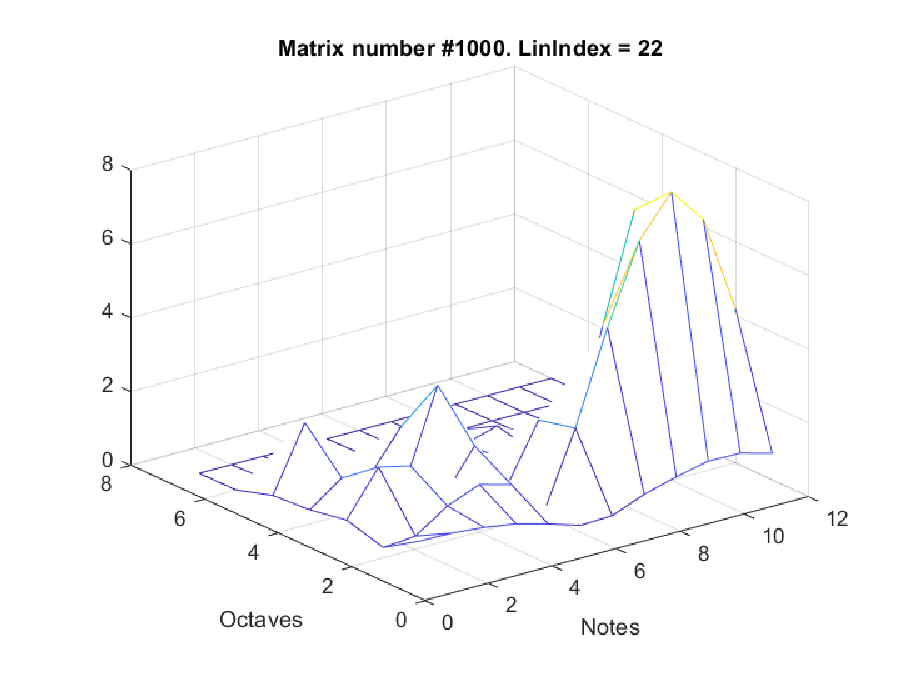
\includegraphics[width=\maxwidth{56.196688409433015em}]{figure_12.eps}
\end{center}
\begin{center}
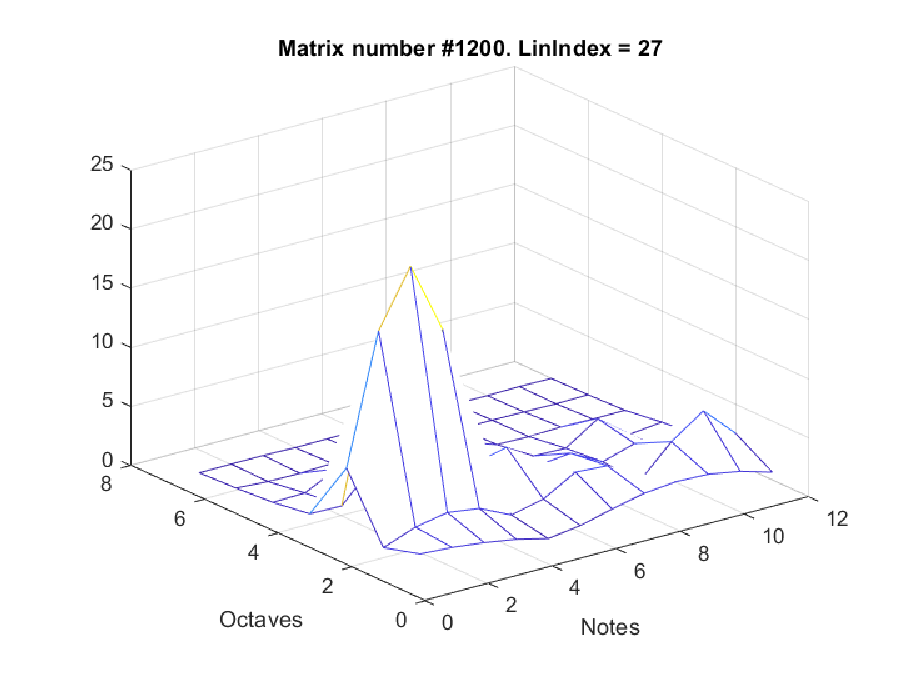
\includegraphics[width=\maxwidth{56.196688409433015em}]{figure_13.eps}
\end{center}
\begin{center}
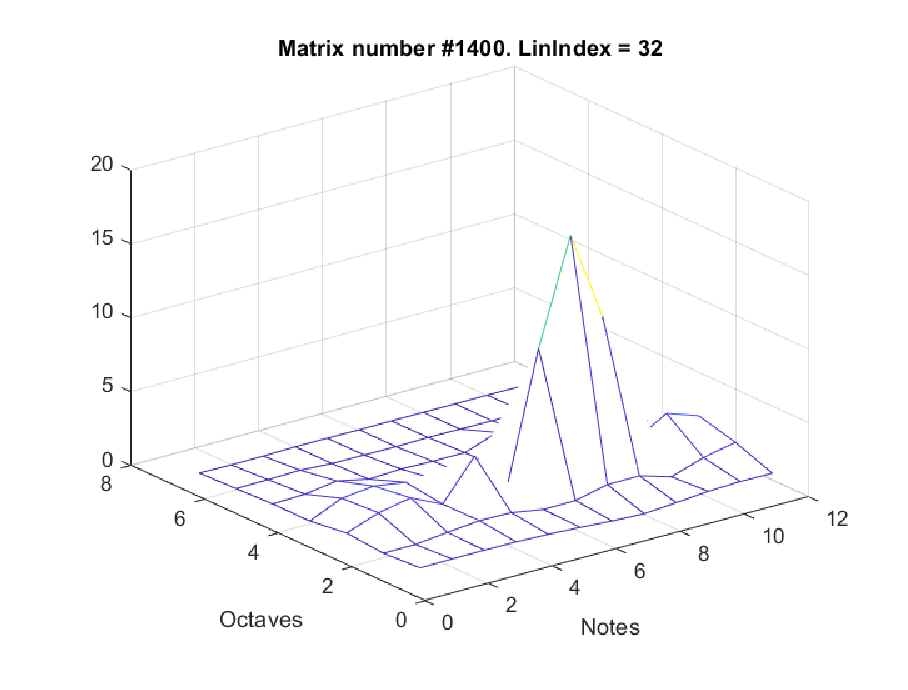
\includegraphics[width=\maxwidth{56.196688409433015em}]{figure_14.eps}
\end{center}
\begin{center}
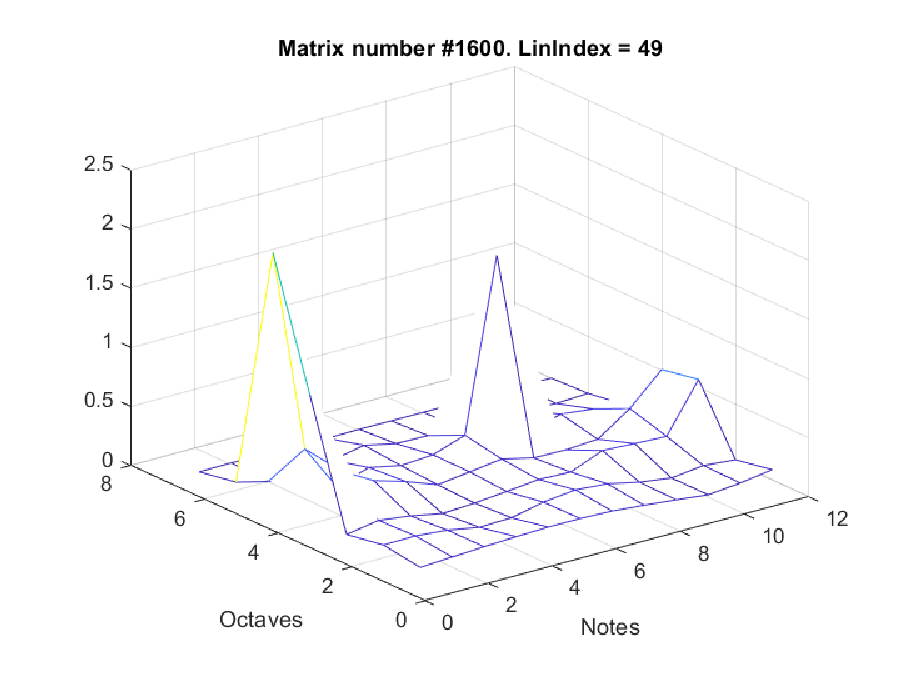
\includegraphics[width=\maxwidth{56.196688409433015em}]{figure_15.eps}
\end{center}
\begin{center}
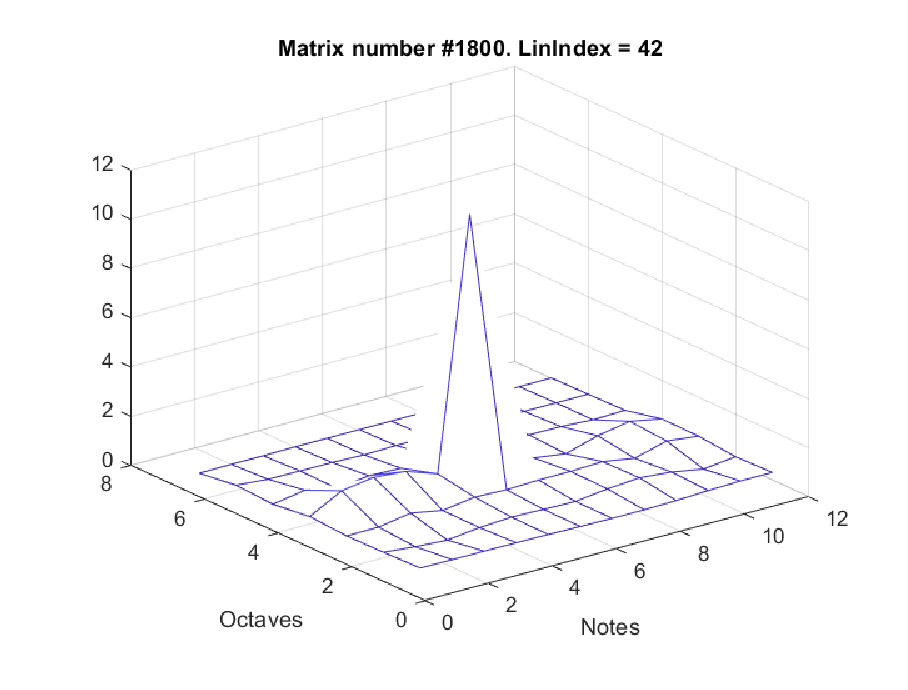
\includegraphics[width=\maxwidth{56.196688409433015em}]{figure_16.eps}
\end{center}
\begin{center}
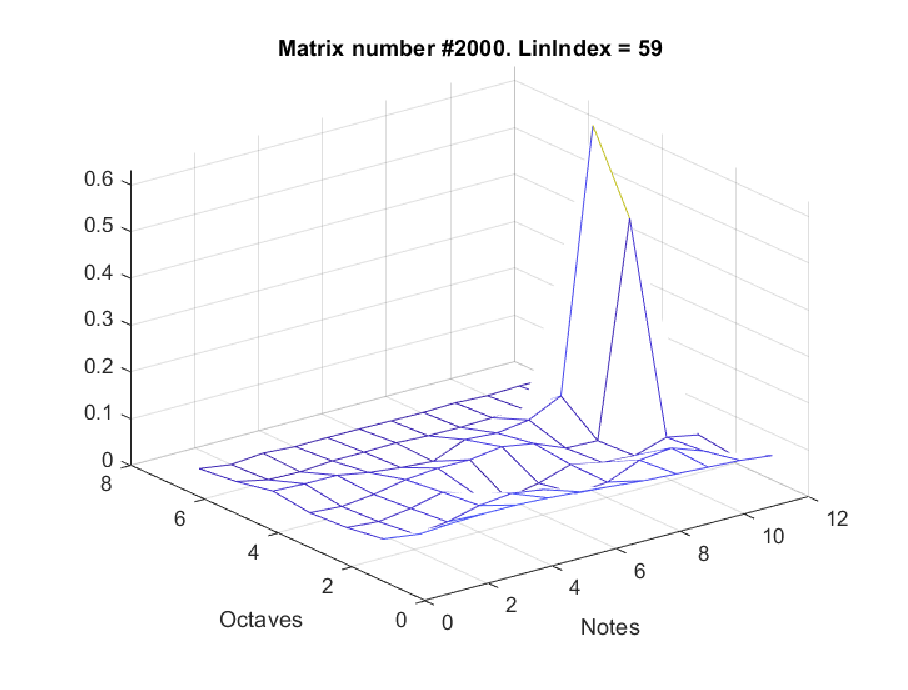
\includegraphics[width=\maxwidth{56.196688409433015em}]{figure_17.eps}
\end{center}
\begin{center}
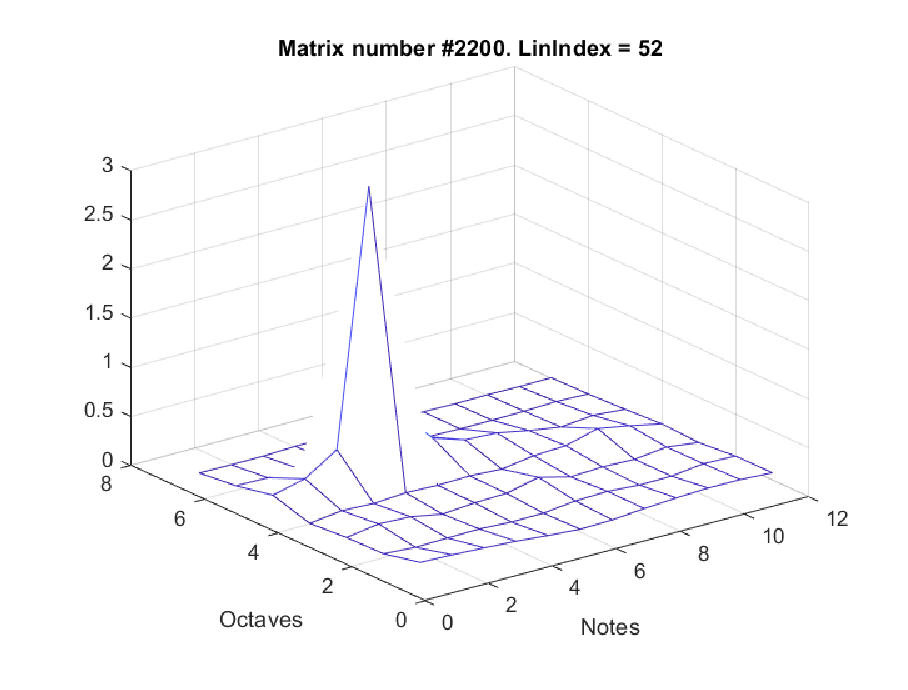
\includegraphics[width=\maxwidth{56.196688409433015em}]{figure_18.eps}
\end{center}
\begin{center}
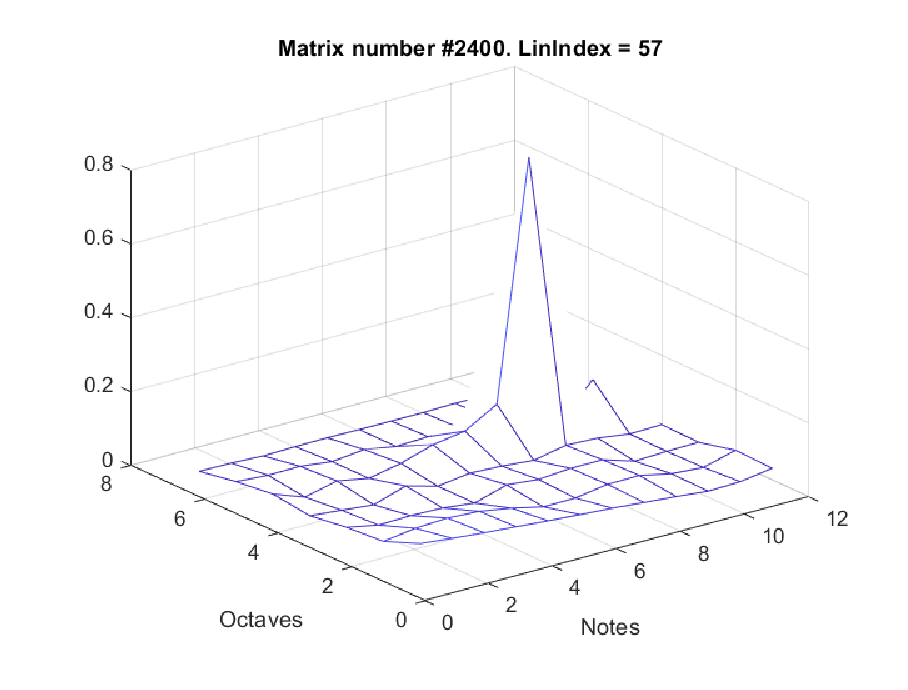
\includegraphics[width=\maxwidth{56.196688409433015em}]{figure_19.eps}
\end{center}
\begin{matlabcode}

t = (1:cuts) * Samples_num / Fs;
plot(t, notes_lin)
xlabel("t, c")
ylabel("Линейный индекс ноты")
title("Определение нот во времени")
\end{matlabcode}
\begin{center}
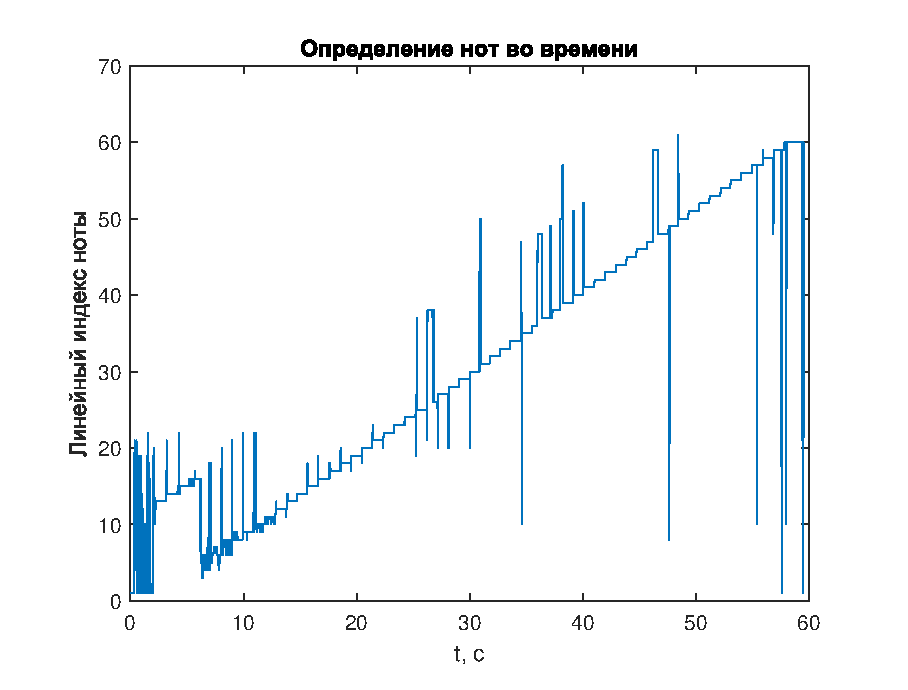
\includegraphics[width=\maxwidth{56.196688409433015em}]{figure_20.eps}
\end{center}


\begin{par}
\begin{flushleft}
Определение нот реальной композиции
\end{flushleft}
\end{par}

\begin{matlabcode}
path = 'D:\Desktop\Studie\Diploma\Audio data\wav\Отрывок композиции для анализа-1.wav';
[y, Fs] = audioread(path);
z = y(:,1);

cuts = floor( length(z) / Samples_num ) - 1;    % Кол-во вірезок по времени
notes_lin = zeros(1, cuts);
k_interp = Fs/Samples_num - 1;
zeros_num = floor( k_interp*Samples_num );
Zer = zeros(zeros_num, 1);
Indexes = floor(L2 * Tab_F / Fs + 1);   % NOT FLAT!!!


for i = 1:cuts
    
    n1 = i*Samples_num;         % Задаю пределы для вырезания участка сигнала
    n2 = (i+1)*Samples_num - 1;
    
    S = z(n1: n2);              % Берем участок сигнала
    S2 = vertcat (Zer, S);      % Интерполируем спектр
    Spec = abs(fft(S2));        % Находим спектр сигнала
    M = Spec(Indexes);          % Заполняем матрицу нот
    
    [Val, Ind] = max(M',[],[1 2], 'linear');   % Нахожу индекс максимума
    
    notes_lin(i) = Ind;         % Сохраняю текущую ноту
    
    if mod(i,200) == 0
        figure(i+1)
        mesh(M);
        xlabel("Notes")
        ylabel("Octaves")
        title("Matrix number #" + string(i) + ". LinIndex = " + string(Ind))
    end
    
end
\end{matlabcode}
\begin{center}
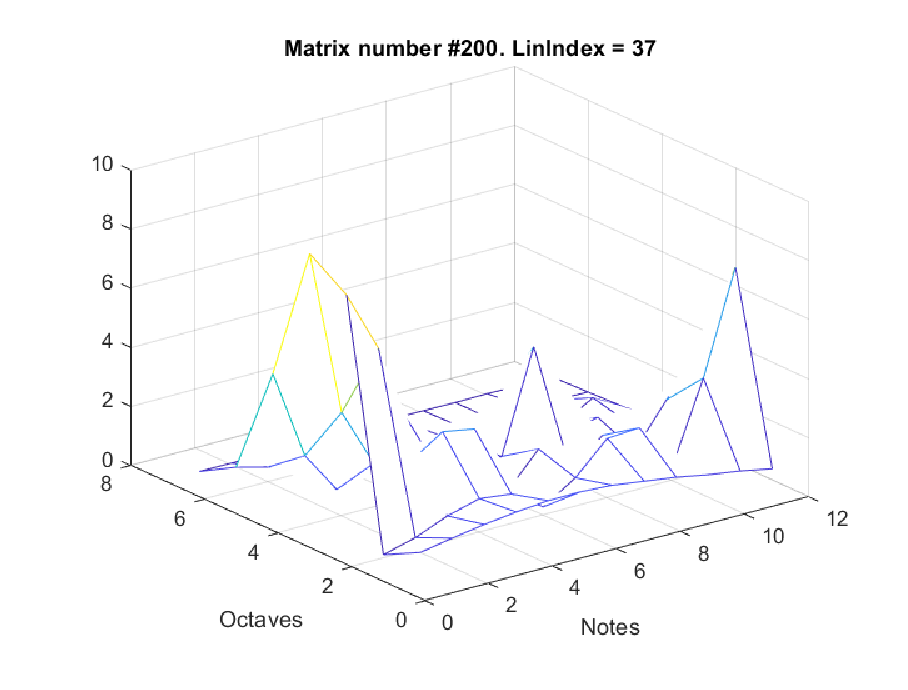
\includegraphics[width=\maxwidth{56.196688409433015em}]{figure_21.eps}
\end{center}
\begin{center}
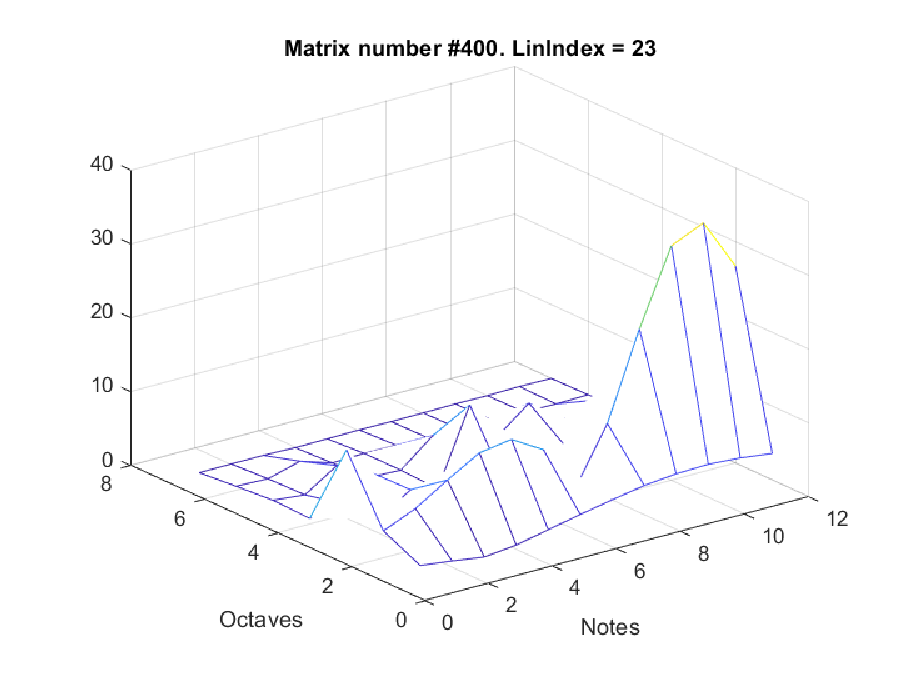
\includegraphics[width=\maxwidth{56.196688409433015em}]{figure_22.eps}
\end{center}
\begin{center}
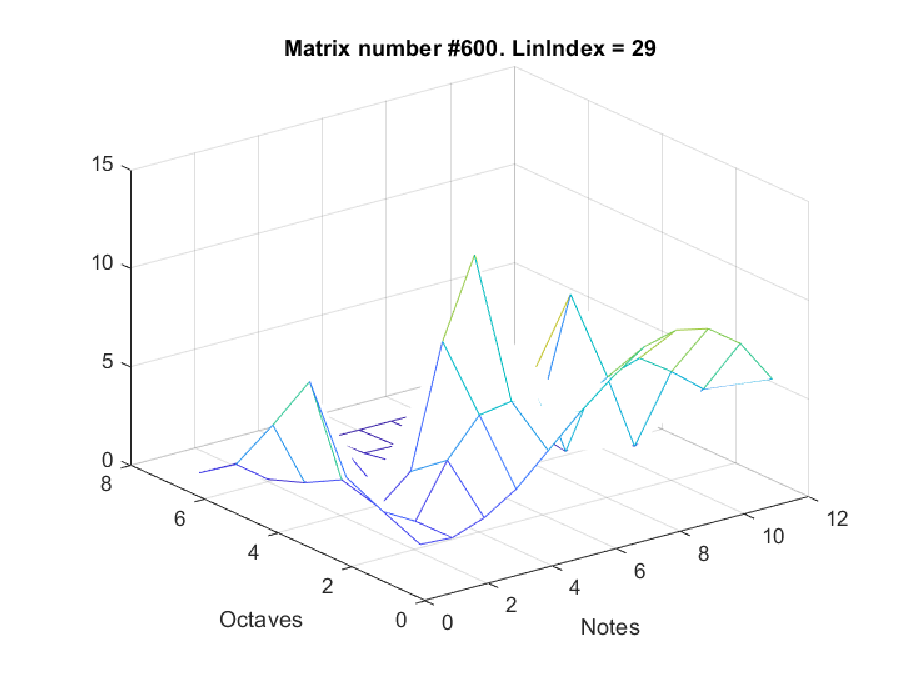
\includegraphics[width=\maxwidth{56.196688409433015em}]{figure_23.eps}
\end{center}
\begin{center}
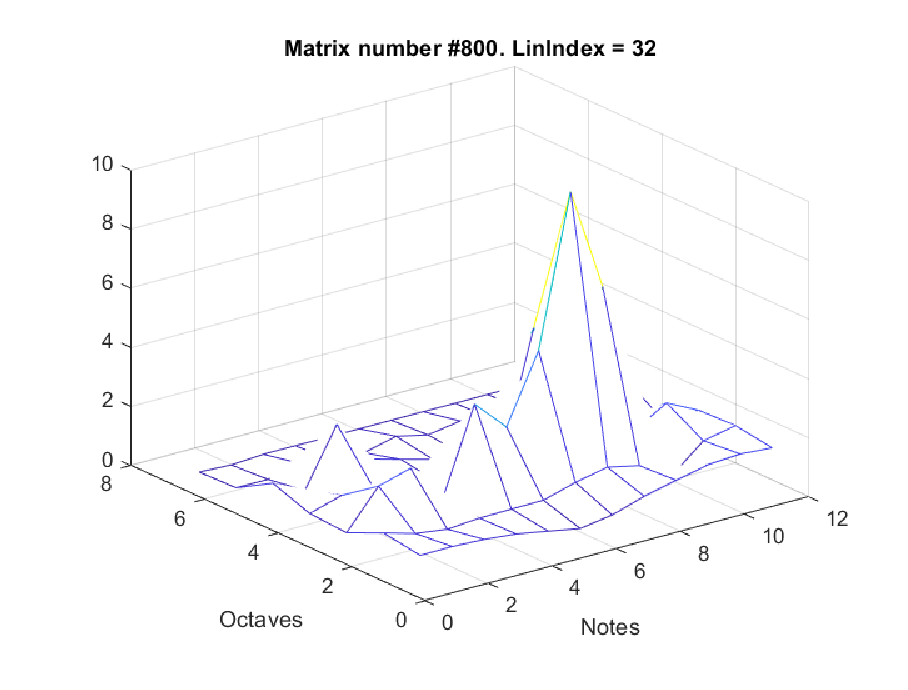
\includegraphics[width=\maxwidth{56.196688409433015em}]{figure_24.eps}
\end{center}
\begin{center}
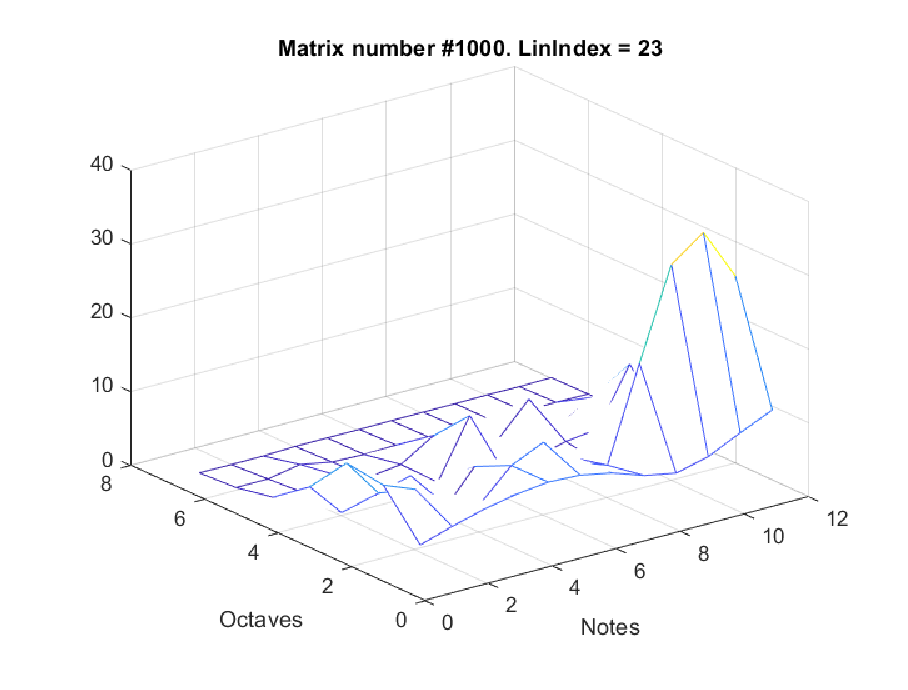
\includegraphics[width=\maxwidth{56.196688409433015em}]{figure_25.eps}
\end{center}
\begin{center}
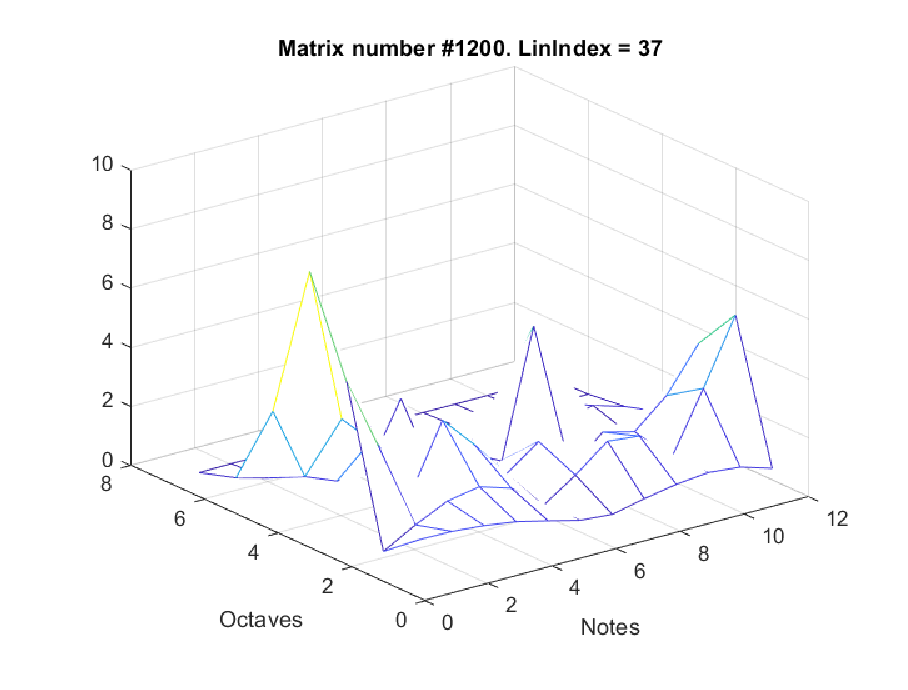
\includegraphics[width=\maxwidth{56.196688409433015em}]{figure_26.eps}
\end{center}
\begin{matlabcode}

t = (1:cuts) * Samples_num / Fs
\end{matlabcode}
\begin{matlaboutput}
t = 1x1385    
    0.0232    0.0464    0.0697    0.0929    0.1161    0.1393    0.1625    0.1858    0.2090    0.2322    0.2554    0.2786    0.3019    0.3251    0.3483    0.3715    0.3947    0.4180    0.4412    0.4644    0.4876    0.5108    0.5341    0.5573    0.5805    0.6037    0.6269    0.6502    0.6734    0.6966    0.7198    0.7430    0.7663    0.7895    0.8127    0.8359    0.8591    0.8824    0.9056    0.9288    0.9520    0.9752    0.9985    1.0217    1.0449    1.0681    1.0913    1.1146    1.1378    1.1610

\end{matlaboutput}
\begin{matlabcode}
plot(t, notes_lin)
title("Определение нот во времени")
xlabel("t, c")
ylabel("Линейный индекс ноты")
\end{matlabcode}
\begin{center}
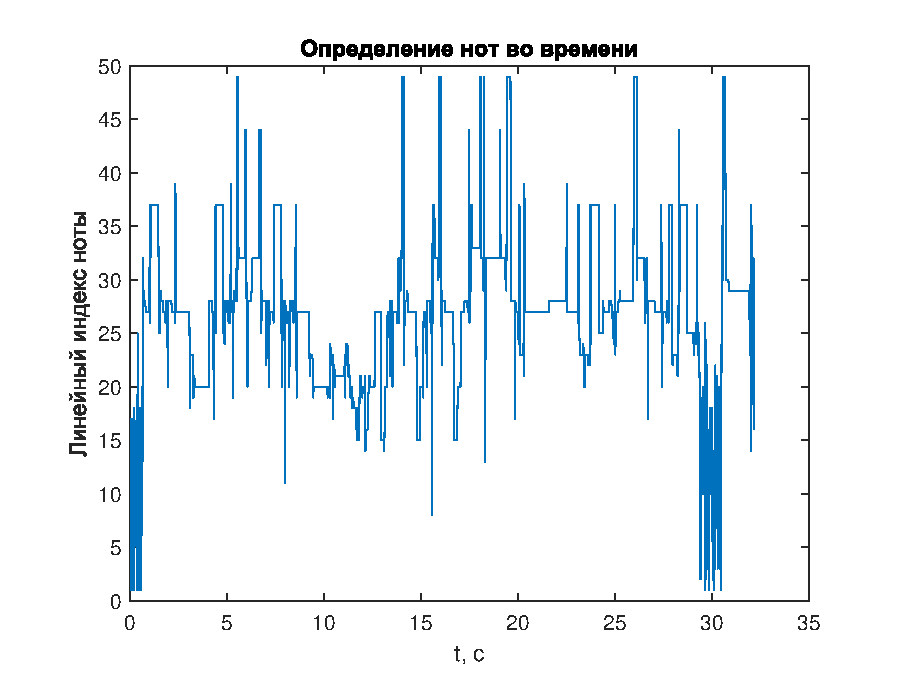
\includegraphics[width=\maxwidth{56.196688409433015em}]{figure_27.eps}
\end{center}


\begin{par}
\begin{flushleft}
Запись полученных нот в текстовый документ
\end{flushleft}
\end{par}

\begin{par}
\begin{flushleft}
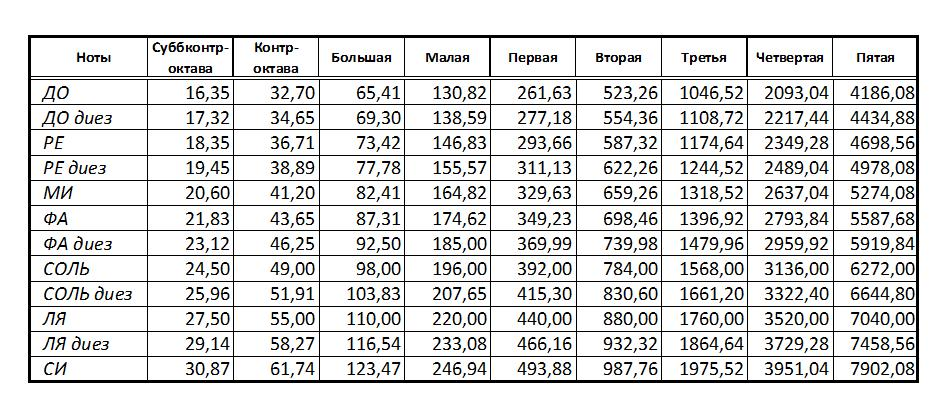
\includegraphics[width=\maxwidth{55.09282488710487em}]{image_2}
\end{flushleft}
\end{par}

\begin{par}
\begin{flushleft}
Заготовленная таблица названий нот и октав
\end{flushleft}
\end{par}

\begin{matlabcode}
Tab_notes = ["C" "C#" "D" "D#" "E" "F" "F#" "G" "G#" "A" "A#" "B"];                  % 12
Tab_octaves = ["Большая" "Малая" "Первая" "Вторая" "Третья" "Четвертая" "Пятая"];    % 7
Tab_duration = ["4" "2" "1" "1/2" "1/4" "1/8" "1/16" "1/32"];                        % 8
\end{matlabcode}

\begin{par}
\begin{flushleft}
Допустим мы получили линейный индекс 29. Знаем заранее что это 5 нота 3тей октавы или "Ми Первой октавы"
\end{flushleft}
\end{par}

\begin{matlabcode}
LinInd = [29 6];

note_num = mod(LinInd, 12)            
\end{matlabcode}
\begin{matlaboutput}
note_num = 1x2    
     5     6

\end{matlaboutput}
\begin{matlabcode}
octave_num = (LinInd - note_num)/12 + 1
\end{matlabcode}
\begin{matlaboutput}
octave_num = 1x2    
     3     1

\end{matlaboutput}
\begin{matlabcode}
note = Tab_notes(note_num)
\end{matlabcode}
\begin{matlaboutput}
note = 1x2 string    
"E"          "F"          

\end{matlaboutput}
\begin{matlabcode}
octave = Tab_octaves(octave_num)
\end{matlabcode}
\begin{matlaboutput}
octave = 1x2 string    
"Первая"     "Большая"    

\end{matlaboutput}
\begin{matlabcode}

duration = ["1/16" "1/4"]
\end{matlabcode}
\begin{matlaboutput}
duration = 1x2 string    
"1/16"       "1/4"        

\end{matlaboutput}

\begin{par}
\begin{flushleft}
Запись данных в текстовый файл
\end{flushleft}
\end{par}

\begin{matlabcode}
T = table(note, octave, duration, 'VariableNames', { 'note', 'octave', 'duration'} )
\end{matlabcode}
\begin{matlabtableoutput}
{
\begin{tabular} {|c|c|c|c|c|c|c|}\hline
\mlcell{ } & \multicolumn{2}{|c|}{\mlcell{note}} & \multicolumn{2}{|c|}{\mlcell{octave}} & \multicolumn{2}{|c|}{\mlcell{duration}} \\ \hline
\mlcell{1} & \mlcell{"E"} & \mlcell{"F"} & \mlcell{"Первая"} & \mlcell{"Большая"} & \mlcell{"1/16"} & \mlcell{"1/4"} \\ 
\hline
\end{tabular}
}
\end{matlabtableoutput}
\begin{matlabcode}
writetable(T, 'MyFile.txt')
\end{matlabcode}


\matlabtitle{НЕ ГОТОВО!!!}

\begin{par}
\begin{flushleft}
Пройдусь по всему сигналу, вырезая из него пачки по 1024 отчета. Из этих пачек я буду находить амплитуды каждой ноты, определять максимальную и говорить, что она является основным тоном. (Учитываем что играется только одна нота)
\end{flushleft}
\end{par}

\begin{par}
\begin{flushleft}
Делаю обезок длинной Samples\_num. Использую перекрытие 1/2 по обрезкам тоже длинной Samples\_num. Передаю спектр обрезка в функцию которая вынимает гармоники и находит максимум. Эта функция возвращает мне частоту с максимальной амплитудой. Я добавляю ее в конец массива. В итоге получаю массив который показывает в какое время какую ноту играли.
\end{flushleft}
\end{par}

\begin{matlabcode}
%{
cur_note = [0 0];
cuts = floor( length(z) / Samples_num ) - 1; % Количество вырезок из сигнала

for i = 1:cuts
    
    if (i > 1)
        L = Samples_num/2;
        S = z(i*Samples_num-L : (i+1)*Samples_num-L - 1);
        F = FillNoteMatrix(S);
        cur_note(end+1) = F;
    end
    
    S = z(i*Samples_num : (i+1)*Samples_num - 1);
    F = FillNoteMatrix(S);
    cur_note(end+1) = F;
    
end
%}
\end{matlabcode}


\begin{par}
\begin{flushleft}
Определяю функцию которая будет избирать из спектра амплитуды, которые находяться по частотам нот и складывать их в M
\end{flushleft}
\end{par}

\begin{par}
\begin{flushleft}
Интерполяцией переведу спектр в такой, что бы шаг частоты был равен 1
\end{flushleft}
\end{par}

\begin{matlabcode}
%{

function F = FillNoteMatrix (S)
    k_interp = Fs/length(S) - 1;
    zeros_num = floor( k_interp*Samples_num);
    Zer = zeros(zeros_num, 1);
    S2 = vertcat (Zer, S);
    
    Spec = abs(fft(S2));        % Получаем спектр с шагом примерно 1Гц
    N = length(Spec);
    N2 = N/2;
    Spec = Spec(1:N2);
    
    for i = 1:length(M)
        
        index = floor( N * Tab_F(i) / Fs ); % Перевод частоты в индекс
        M(i) = Spec(index);
       
    end
    
    F; index = max(M);
    
end
%}
\end{matlabcode}

\end{document}
